\documentclass[12pt,a4paper,titlepage]{article}
\usepackage[utf8]{inputenc}
\usepackage{amsmath}
\usepackage{amsfonts}
\usepackage{amssymb}
\usepackage{graphicx}
\usepackage{tabularx}
\usepackage[left=2cm,right=2cm,top=2cm,bottom=2cm]{geometry}
\usepackage{titlesec}
\usepackage{listings}


\newcommand{\footlabel}[2]{%
    \addtocounter{footnote}{1}%
    \footnotetext[\thefootnote]{%
        \addtocounter{footnote}{-1}%
        \refstepcounter{footnote}\label{#1}%
        #2%
    }%
    % $^{\ref{#1}}$%
}

\newcommand{\footref}[1]{%
    $^{\ref{#1}}$%
}

\newcounter{normalfootc}
\renewcommand{\footnote}[1]{%
    \footlabel{footsaferefiwontuse\thenormalfootc}{#1}%
    \addtocounter{normalfootc}{1}%
}

\graphicspath{{images/}}

\usepackage[hypcap]{caption}
\usepackage[
	pdfusetitle, 
	hidelinks
]{hyperref}
\hypersetup{ 
    bookmarksnumbered=true,     
    bookmarksopen=true,         
    bookmarksopenlevel=2,         
    pdfstartview=Fit,           
    pdfpagemode=UseOutlines,    % this is the option you were lookin for
    pdfpagelayout=SinglePage
    }
    
\usepackage{float}

\author{SDP Group 12}
\title{Technical Specification}

\begin{document}
\maketitle

%Group final report No more than 12 pages, worth 16 (out of 50) marks

%Reports have three purposes: to provide sufficient information to assess your work; to document for the group and yourself your design and what you have done; and to provide useful information for anyone who wants to build on what you have done in future. Reports may contain detailed appendices beyond the page limit, particularly in aid of the last two goals; but markers are not required to read these appendices. A common mistake is to overuse the appendices— figures, tables, or other material that explains your work belongs in the main report, not an appendix. Large illustrations will not count towards the page limits.


\section{Introduction}

The aim of this project was to create a robot that would play a simplified version of 2-a-side football. We were recommended to use the provided Arduino Uno (Xino RF) board and LEGO pieces, a vision feed of the testing area (pitch), and computers to connect the two and implement any further logic.

This report will examine the decisions made in the design of each part and their impacts. Furthermore it will explain the principles our work relies on.


\subsection{Work Distribution and Management}
Overall the group was efficiently split into subgroups working on specific tasks. All team members have made contributions to the outcome of the project, though the weights vary.

Furthermore, many tasks were shared with Group 11, and large contributions introduced by teamwork between the two halves of the team.


%\subsection{Planning}
%Mostly worked on planning.
%
%\subsection{Joel Hutton}
%Responsible for hardware.
%
%\subsection{Hugh McGrade}
%Leader of planning development.
%
%\subsection{Margus Lind}
%All around
%
%\subsection{Sanchit Gupta}
%Mostly worked on vision.
%
%\subsection{Simeon "King of Calibration" Ivanov}
%Leader of vision development.

\section{Vision}

\subsection{Requirements}
You'll need the following python packages to successfully run the vision:

\begin{description}
\item \texttt{Polygon2} Polygon is a python package that handles polygonal shapes in 2D. 
\item \texttt{argparse} Python command-line parsing library
\item \texttt{pyserial} Python Serial Port Extension
\item \texttt{numpy} Array processing for numbers, strings, records, and objects.
\item \texttt{openCV} OpenCV-Python is the Python API of OpenCV. It combines the best qualities of OpenCV C++ API and Python language.
\end{description}

To install them run these commands in the terminal:

\shellcmd{pip install --user Polygon2==2.0.6} \\
\shellcmd{pip install --user argparse==1.3.0} \\
\shellcmd{pip install --user pyserial==2.7} \\
\shellcmd{pip install --user numpy}  

You can also learn how to install openCV from the following link:
\url{http://docs.opencv.org/2.4/doc/tutorials/introduction/linux_install/linux_install.html}

\subsection{Usage}
Before using the vision system, you can have a look at the vision feed by typing "xawtv" in the command prompt. This will launch only the vision feed, where you can experiment with the different settings.

In order to launch our vision system, you'll need to run the main vision file (python vision.py). At first, a window for the automatic colour calibration will pop out. You'll need to follow the instructions as printed in the terminal. The calibration goes through all the colours that are used for the vision (‘red’, ‘yellow’, ‘blue’, ‘green’, ‘pink’) and requires multiple clicks for each one of them to get their thresholds. You need to press the ‘q’ button after each calibrated colour. If you want to skip the calibration you can simply press the ‘Esc’ key and the vision will use the previously saved calibrations.

After this, the vision will be launched. There will be a window named ‘Filter output’, where you can see the vision feed with objects drawn on it representing the robots and the ball (if they are found). Robots will be represented by an inner circle for the team colour (‘yellow’ or ‘blue’), an outer circle identifying which of the two teammates it is (‘pink’ or ‘green’) and an arrow giving the direction of the robot.  The red ball is simply shown by drawing a red circle around it. You’ll also notice two other windows containing several trackbars. These trackbars are for filters that you can add to the output feed. There are filters to show only specific colours, or to different effects to the frame.

When the vision is running, it will provide the coordinates of all found objects, their orientation and velocity relative to the previous taken frame. These objects are returned as a dictionary and are passed onto the planner.



\section{Planning}
\lstset{language=Python, showstringspaces=false}


\begin{figure}[H]
\centering
\begin{subfigure}{.5\textwidth}
\centering
\begin{tikzpicture}

\tikzset{
    right angle quadrant/.code={
        \pgfmathsetmacro\quadranta{{1,1,-1,-1}[#1-1]}     % Arrays for selecting quadrant
        \pgfmathsetmacro\quadrantb{{1,-1,-1,1}[#1-1]}},
    right angle quadrant=1, % Make sure it is set, even if not called explicitly
    right angle length/.code={\def\rightanglelength{#1}},   % Length of symbol
    right angle length=2ex, % Make sure it is set...
    right angle symbol/.style n args={3}{
        insert path={
            let \p0 = ($(#1)!(#3)!(#2)$) in     % Intersection
                let \p1 = ($(\p0)!\quadranta*\rightanglelength!(#3)$), % Point on base line
                \p2 = ($(\p0)!\quadrantb*\rightanglelength!(#2)$) in % Point on perpendicular line
                let \p3 = ($(\p1)+(\p2)-(\p0)$) in  % Corner point of symbol
            (\p1) -- (\p3) -- (\p2)
        }
    }
}


\node  (robot)  [draw, inner sep=5] at (0,-1) {ROBOT};
\node  (target)  [draw,inner sep=5] at (0,5) {TARGET};
\draw  (robot) [-triangle 60] edge (target);

\node (o1)[draw] at (-2,1) {$O_1$};
\coordinate (p1) at (0,1) {};
\draw  (o1) [<->] edge node[midway, below] {$d_1$} (p1);
\draw [right angle symbol={robot}{p1}{o1}];
    

\node (o2)[draw] at (1,3) {$O_2$};
\coordinate (p2) at (0,3) {};
\draw  (o2) [<->] edge node[auto] {$d_2$} (p2);
\draw [right angle symbol={robot}{p2}{o2}];

\end{tikzpicture}
\caption{Detection}
\label{fig:obstacle_detection}
\end{subfigure}%
\begin{subfigure}{.5\textwidth}
\centering
\begin{tikzpicture}
  
\tikzset{
    right angle quadrant/.code={
        \pgfmathsetmacro\quadranta{{1,1,-1,-1}[#1-1]}     % Arrays for selecting quadrant
        \pgfmathsetmacro\quadrantb{{1,-1,-1,1}[#1-1]}},
    right angle quadrant=1, % Make sure it is set, even if not called explicitly
    right angle length/.code={\def\rightanglelength{#1}},   % Length of symbol
    right angle length=2ex, % Make sure it is set...
    right angle symbol/.style n args={3}{
        insert path={
            let \p0 = ($(#1)!(#3)!(#2)$) in     % Intersection
                let \p1 = ($(\p0)!\quadranta*\rightanglelength!(#3)$), % Point on base line
                \p2 = ($(\p0)!\quadrantb*\rightanglelength!(#2)$) in % Point on perpendicular line
                let \p3 = ($(\p1)+(\p2)-(\p0)$) in  % Corner point of symbol
            (\p1) -- (\p3) -- (\p2)
        }
    }
}

\node  (robot)  [draw, inner sep=5] at (0,-1) {ROBOT};
\node  (target)  [draw,inner sep=5] at (0,5) {TARGET};
\draw  (robot) [dotted, -open triangle 60] edge node [sloped, below left ]{original path} (target);

\node (obstacle)[draw] at (1,3) {$O_2$};
\draw [dashed, shorten >=-3cm,shorten <=-3cm] ($(robot)!(obstacle)!(target)$) -- (obstacle);

\draw [right angle symbol={robot}{$(robot)!(obstacle)!(target)$}{obstacle}];
\coordinate (new) at (-1.5,3) {};

\path (robot) [-triangle 60] edge node [sloped,below] {corrected path} (new)
(new) [-triangle 60] edge (target);

\draw[decorate,decoration={brace,raise=2pt,amplitude=2pt}] (obstacle)  -- node[below=3pt]{$d_{min}$} (new) ;

\end{tikzpicture}
\caption{Avoidance}
\label{fig:obstacle_avoidance}
\end{subfigure}
\caption{Handling Obstacles}
\label{handling_obstacle}
\end{figure}



\subsection{Design}

The planner uses a system of goals and actions. Goals define an overall strategy in a given situation leading to a particular aim. Actions define one instruction given to the robot with preconditions for its execution. Goals are composed of a sequence of actions. A goal object selects the next action required to achieve its aim by traversing its ordered list of actions and evaluating their preconditions.

In the implementation, all goals and actions are derived from their respective super classes. These are defined as follows:

\begin{figure}[p]
	\begin{center}
          \includegraphics[width=1.0\linewidth]{Goal}
          \caption{Definition of super class for goals}
	\end{center}
\end{figure}


\begin{figure}[p]
	\begin{center}
          \includegraphics[width=1.0\linewidth]{Action}
          \caption{Definition of super class for actions}
	\end{center}
\end{figure}


The planner makes its decision based on only on the world state passed to it. This is described by an instance of the  class passed to the planner. This object's state is updated by passing a new set of positions (as a dictionary of vectors) to the \texttt{update\_positions} method of \texttt{World}. The \texttt{World} class describes the state of the world from the vision, including position vectors for the robots, the ball and the goals. The \texttt{World} class and its associated classes also provide methods on their data providing the planner with information about the world. Further utility functionality can be found in ``utils.py''

The overall planner is used by calling \texttt{plan\_and\_act(world)}.
This selects a goal based on the given world state  using its \texttt{get\_goal()} method. From this goal an action is generated using \texttt{generate\_action()}. The method then runs (using \texttt{actuate(action)}) and returns a delay giving the time until the planner should be run again.

In order to succeed, the planner must be able to detect obstacles on the path of a robot's movement and on the path of a pass or shot on goal. Having established a location and target, the planner checks for obstacles as follows:

\begin{figure}[H]
\begin{center}
\begin{tikzpicture}

\tikzset{
    right angle quadrant/.code={
        \pgfmathsetmacro\quadranta{{1,1,-1,-1}[#1-1]}     % Arrays for selecting quadrant
        \pgfmathsetmacro\quadrantb{{1,-1,-1,1}[#1-1]}},
    right angle quadrant=1, % Make sure it is set, even if not called explicitly
    right angle length/.code={\def\rightanglelength{#1}},   % Length of symbol
    right angle length=2ex, % Make sure it is set...
    right angle symbol/.style n args={3}{
        insert path={
            let \p0 = ($(#1)!(#3)!(#2)$) in     % Intersection
                let \p1 = ($(\p0)!\quadranta*\rightanglelength!(#3)$), % Point on base line
                \p2 = ($(\p0)!\quadrantb*\rightanglelength!(#2)$) in % Point on perpendicular line
                let \p3 = ($(\p1)+(\p2)-(\p0)$) in  % Corner point of symbol
            (\p1) -- (\p3) -- (\p2)
        }
    }
}


\node  (robot)  [draw, inner sep=5] at (0,0) {ROBOT};
\node  (target)  [draw,inner sep=5] at (0,5) {TARGET};
\draw  (robot) [-triangle 60] edge (target);

\node (o1)[draw] at (-2,2) {$O_1$};
\coordinate (p1) at (0,2) {};
\draw  (o1) [<->] edge node[midway, below] {$d_1$} (p1);
\draw [right angle symbol={robot}{p1}{o1}];
    

\node (o2)[draw] at (1,3) {$O_2$};
\coordinate (p2) at (0,3) {};
\draw  (o2) [<->] edge node[auto] {$d_2$} (p2);
\draw [right angle symbol={robot}{p2}{o2}];


\end{tikzpicture}
\caption{Diagram of planner's approach to obstacle avoidance, O_i is an obstacle if \(d_i > THRESHOLD\) }
\end{center}
\end{figure}

By finding the distance of each object from the path and using a constant threshold, the planner establishes whether or not, and if so which, objects will be obstacles to a given path. If an obstacle is found, the planner must, if possible, generate a new path avoiding the obstacle. This is done using the line perpendicular to the path passing through the obstacle. The planner iterates over points at fixed distances along the line, working outwards from the original path, testing for obstacles on this corrected path. This produces a minimal path avoiding the obstacle.

\begin{figure}[H]
\begin{center}

\begin{tikzpicture}
  
\tikzset{
    right angle quadrant/.code={
        \pgfmathsetmacro\quadranta{{1,1,-1,-1}[#1-1]}     % Arrays for selecting quadrant
        \pgfmathsetmacro\quadrantb{{1,-1,-1,1}[#1-1]}},
    right angle quadrant=1, % Make sure it is set, even if not called explicitly
    right angle length/.code={\def\rightanglelength{#1}},   % Length of symbol
    right angle length=2ex, % Make sure it is set...
    right angle symbol/.style n args={3}{
        insert path={
            let \p0 = ($(#1)!(#3)!(#2)$) in     % Intersection
                let \p1 = ($(\p0)!\quadranta*\rightanglelength!(#3)$), % Point on base line
                \p2 = ($(\p0)!\quadrantb*\rightanglelength!(#2)$) in % Point on perpendicular line
                let \p3 = ($(\p1)+(\p2)-(\p0)$) in  % Corner point of symbol
            (\p1) -- (\p3) -- (\p2)
        }
    }
}

\node  (robot)  [draw, inner sep=5] at (0,-1) {ROBOT};
\node  (target)  [draw,inner sep=5] at (0,5) {TARGET};
\draw  (robot) [dotted, -open triangle 60] edge node [sloped, below left ]{original path} (target);

\node (obstacle)[draw] at (1,3) {$O_2$};
\draw [dashed, shorten >=-1.5cm,shorten <=-2.5cm] ($(robot)!(obstacle)!(target)$) -- (obstacle);

\draw [right angle symbol={robot}{$(robot)!(obstacle)!(target)$}{obstacle}];
\coordinate (new) at (-1.5,3) {};

\path (robot) [-triangle 60] edge node [sloped,below] {corrected path} (new)
(new) [-triangle 60] edge (target);

\draw[decorate,decoration={brace,raise=2pt,amplitude=2pt}] (obstacle)  -- node[below=3pt]{$d_{min}$} (new) ;

\end{tikzpicture}

\caption{Diagram demonstrating obstacle avoidance algorithm}
\end{center}
\end{figure}

\subsection{Implementation}

The attacker robot's goals and their respective actions are explained in \autoref{tbl:goals-actions}.
The planner chooses a goal based on ball position, as explained in \autoref{tbl:goals}.

\begin{table}[H]
\centering
\begin{tabularx}{\textwidth}{l l X}
\toprule
\textbf{Goal} & \textbf{Action} & \textbf{Preconditions} \\ 
\midrule

AttackPosition & TurnToDefenderToReceive & Attacker in score zone \\ 
&GoToScoreZone & Attacker is facing score zone  \\ 
&TurnToScoreZone & None \\
\midrule

Score & Shoot & Attacker has ball and attacker can score \\ 
& TurnToGoal & Attacker has ball \\ 
\midrule

GetBall & GrabBall & Attacker can catch ball and attacker's grabbers open \\ 
& GoToGrabStaticBall & Ball static, attacker facing ball, attacker's grabbers open \\ &OpenGrabbers & Ball in attacker's grab range, attacker's grabbers closed \\ 
&GoToBallOpeningDistance & Attacker is facing ball \\
&TurnToBall & None \\ 
\midrule

AttackerBlock & TurnToBlockingAngle & Attacker in blocking position \\ 
& GoToBlockingPosition & Attacker is facing blocking position \\ 
& TurnToFaceBlockingPosition & None \\ 
\bottomrule
\end{tabularx}
\caption{Actions and Preconditions by Goals}
\label{tbl:goals-actions}
\end{table}


\begin{table}[H]
\centering
\begin{tabular}{ l l}
\toprule
\textbf{Robot in possession} & \textbf{Goal} \\ \midrule
Our attacker & Score \\
Our defender & AttackPosition \\
Their attacker & AttackPosition \\
Their defender & AttackerBlock \\
Ball free & GetBall \\ \bottomrule
\end{tabular}
\caption{Goals chosen dependent on ball position}
\label{tbl:goals}
\end{table}

\subsection{Extensibility}

Extending the planner is simply a case of adding goals and actions then adding the logic to select these in \texttt{select\_goal(world)}. Any new goals or actions should subclass Goal and Action respectively and override methods were stated.

In actions, the logic for performing should be placed in \texttt{perform(comms)}. This method is passed a \texttt{CommsManager} object through which the robot can be sent instructions. No more than one call should be made to this object in any given action. A new action should also override \texttt{get\_delay} giving an appropriate delay (in seconds) before the planner should run again. New actions can also have preconditions defined in a variable \texttt{preconditions}.

In goals, it may only be neccessary to write a Goal subclass with an ordered list of actions (from last to first). Otherwise the \texttt{generate\_action()} method can be overriden but similar logic should be followed.

\subsection{Integration}

An instance of the \texttt{Planner} is kept by the ``main.py'' script. Based on the delays given by the planner, it calls the planner at varying intervals, passing it the latest world model provided by the vision. The planner uses a \texttt{CommsManager} object to make control the robot.



\section{Communications}
Communications between the arduino and computer are done over the supplied RF link. The frequency is set to the group frequency specified. Further the optional encryption was enabled and the PAN ID set to 6810.

Data is send to and from the devices in packets, the basic form of a packet is: \\
`\verb$<target><source><data><checksum>\r\n$'\\ 
\texttt{<target>} and \texttt{<source>} are the ASCII character `1' for the group 11 robot, the ASCII character `2' for the group 12 robot, and the ASCII character `c' for the computer. For robot to computer messages, the targets `d' and `e' are also valid, used to send debug and error messages respectively. \texttt{<data>} is the base64 encoded binary message, and \texttt{<checksum>} a checksum of the preceding message.  The base64 encoding
does not use padding bytes, but is otherwise standard.

The checksum consists of 2 characters, which are calculated as the checksum of all characters at even (starting 0) and odd indices respectively, including \texttt{<target>} and \texttt{<source>}. These checksums are done by retrieving the value from 0-63 of the character in base64 encoding, XORing these together. 
The resulting value from 0-63 is then encoded back into a base64 character.

For example, the checksum of `\texttt{dt6bas2}' is `\texttt{La}'.

Devices ignores all packets not addressed to it, as well as malformed packets (including incorrect checksum). Upon receipt of a packet, the device sends an acknowledgement. An acknowledgement packet has the form `\verb%<target>$<checksum>\r\n%'. An acknowledgement packet is not itself acknowledged.

The computer side will resend packets which have not received an acknowledgement. The Arduino side does not, and discards packets which are longer than the internal buffer (60 bytes). To prevent flooding, only the previously sent packet is resent. This suits the application well, as previously sent packets contain instructions to the robot which are superseded by the more recent one.

\subsection{Bytecode}

The data received by the Arduino from the controller is interpreted as a sequence of bytecode instructions. Each instruction starts with a single byte opcode specifying the instruction itself, followed by a number of bytes for the argument of the instruction. The number of bytes the argument used depend on the instruction itself (See the arguments column below; An instruction with a single \verb$uint16_t$ argument will take 2 bytes for its arguments).

%\noindent
\begin{table}[H]

\begin{tabularx}{\textwidth}{rlX}
    Opcode & Arguments & Description \\
    \hline
    \texttt{0x00} & time (\texttt{uint16\_t}) &
        Waits for the given time \\
    \texttt{0x01} & time (\texttt{uint16\_t}) &
        Brakes for the given time \\
    \texttt{0x02} & distance (\texttt{int16\_t}) &
        Moves the given distance to the right (or neg. left) \\
    \texttt{0x03} & angle (\texttt{int16\_t}) &
        Spins the given (possibly negative) angle clockwise \\
    \texttt{0x04} & time (\texttt{uint16\_t}) &
        Activates the kicker for the given time \\
    \texttt{0x06} & \textit{none} &
        Opens the grabbers \\
    \texttt{0x07} & \textit{none} &
        Closes the grabbers \\
    \texttt{0x09} & speed (\texttt{uint8\_t}) &
        Sets the global speed modifier (value from 0-255) \\
%    \texttt{0x0a} & distance (\texttt{int16_t}), radius (\texttt{int16_t}) &
%        Moves the specified distance on an arc with the given radius in front
%        of the robot \\
\end{tabularx}
\end{table}

Times are given in milliseconds, distances in mm and angles in minutes.  The arguments are read directly from instruction sequence memory as the given type, and the next command starts after the current one finishes. Numbers are encoded in little-endian.

The instructions, when received, are compiled by the Arduino into low-level commands, and inserted at the earliest possible point in the low-level command queue.

\subsection{Low-Level Commands}

The arduino internally maintains a queue of low-level commands which capture what the robot is currently doing. Once a command finishes, the Arduino immediately moves on to the next. Structurally, low-level commands work similarly to high-level ones. They start with an opcode, depending on which some arguments may follow. The available low-level commands are:

\begin{table}[H]
\begin{tabularx}{\textwidth}{rlX}
    Opcode & Arguments & Description \\
    \hline
    \texttt{0x00} & time (\texttt{uint16\_t}) &
        Waits for the given time \\
    \texttt{0x01} & time (\texttt{uint16\_t}) &
        Brakes for the given time \\
    \texttt{0x02} & time (\texttt{uint16\_t}) &
        Opens the grabbers for the given time \\
    \texttt{0x03} & time (\texttt{uint16\_t}) &
        Closes the grabbers slowly for the given time \\
    \texttt{0x04} & time (\texttt{uint16\_t}) &
        Closes the grabbers quickly for the given time \\
    \texttt{0x05} & time (\texttt{uint16\_t}) &
        Activates the kicker for the given time \\
    \texttt{0x08} & distance (\texttt{int16\_t}) &
        Moves right by the given distance \\
    \texttt{0x09} & angle (\texttt{int16\_t}) &
        Spins clockwise by the given angle \\
    \texttt{0x0b} & speed (\texttt{uint8\_t}) &
        Sets the global speed modifier to the given value \\
%    \texttt{0x0c} & distance (\texttt{int16_t}), front wheel weight (\texttt{uint16_t}), back wheel weight (\texttt{uint16_t}) &
%        Moves the given distance, with the speed of the front and back wheels being in the specified proportion (used for arc movement) \\
    \texttt{0x7f} & \textit{none} & Does nothing \\
\end{tabularx}
\end{table}

Further, the most significant bit of a low-level commands opcode signifies if this command is interruptible or not. If it is 1, the command is not interruptible.

The Arduino periodically updates the instruction list to decrease the time argument of the current instruction by the time passed, or, if the instruction is finished, moving onto the next one. If a new command sequence arrives, it is inserted in place of the first interruptible command in the sequence, with this, and all later commands being discarded. This ensures that non-interruptible commands are always run, and are run even if they consist of complex sequences which should not be interrupted. This is also the main reason for a no-op existing; it allows separating multiple sequences of non-interruptible commands.

Instructions setting values relating to the communications test are set immediately, and the Arduino moves on to the next instruction. The send instruction \texttt{0xf2} suspends normal operation and executes a writing the buffer to the I$^2$C port with the previously set delay.

\section{Hardware}

\begin{figure}[H]
\begin{subfigure}{.45\textwidth}
\centering
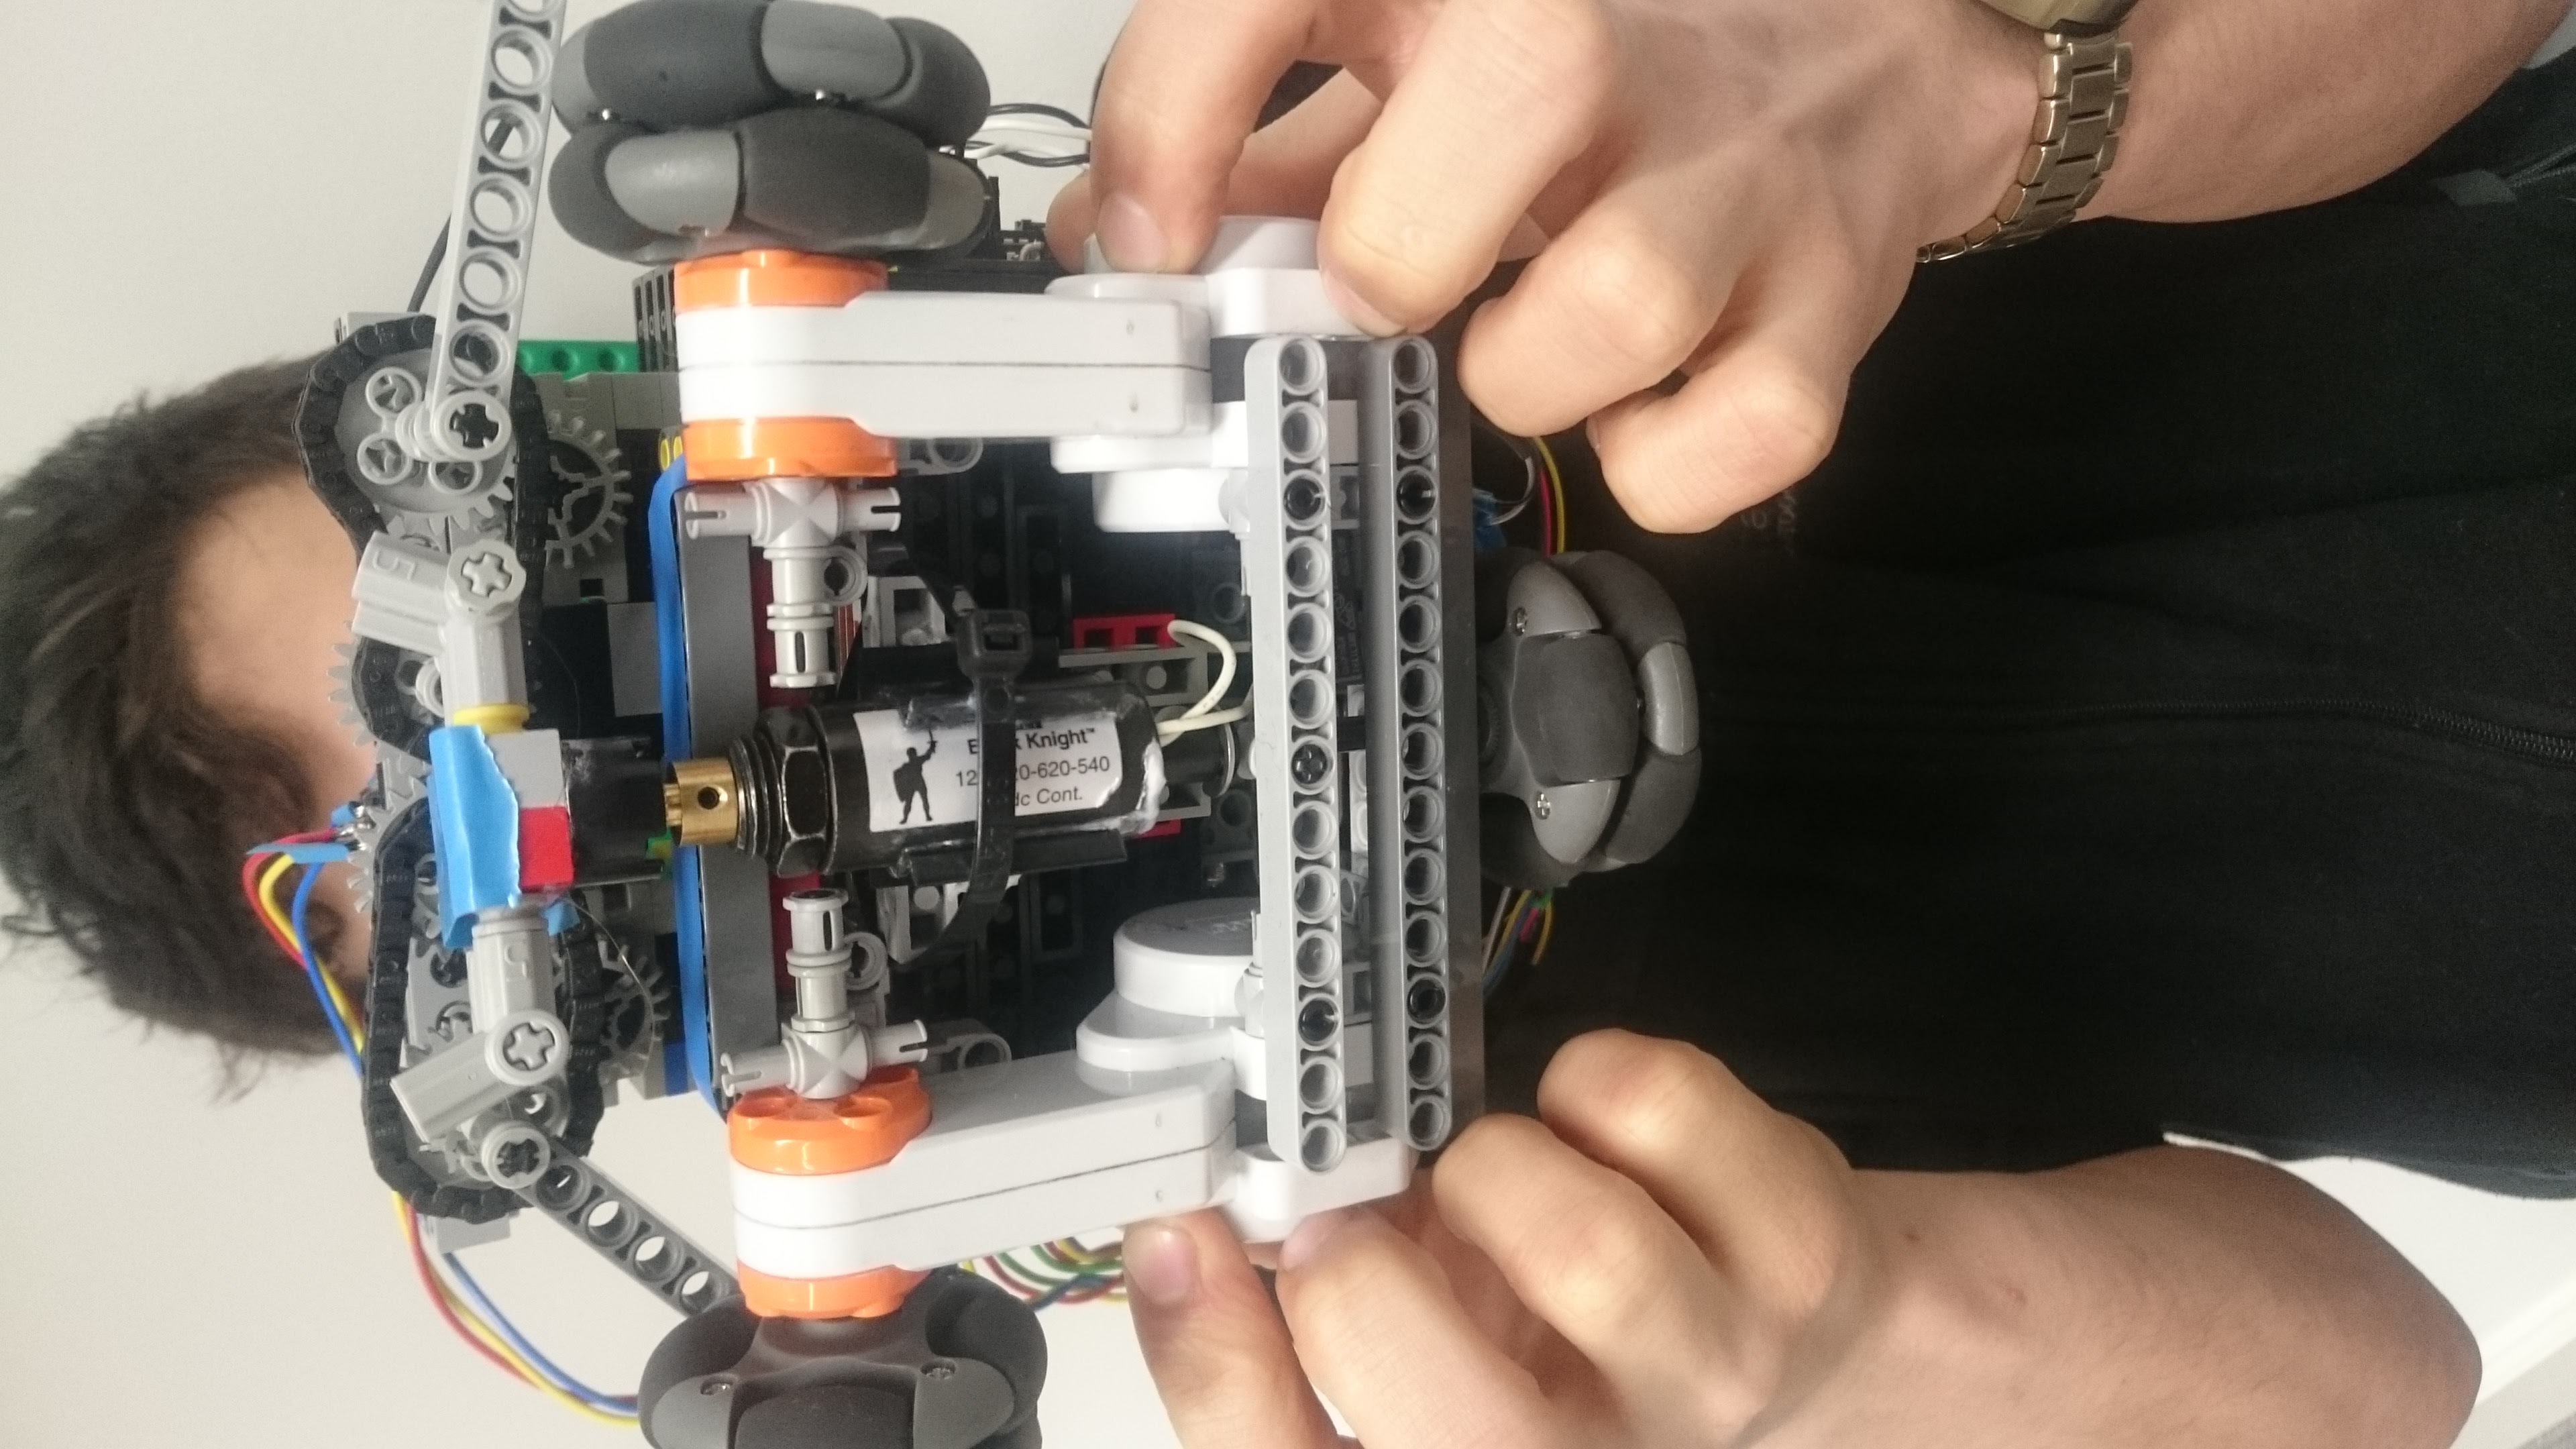
\includegraphics[width=.95\textwidth]{DSC_0036.jpg}
\caption{Wheelbase}
\label{pic:wheelbase}
\end{subfigure}
\begin{subfigure}{.45\textwidth}
\centering
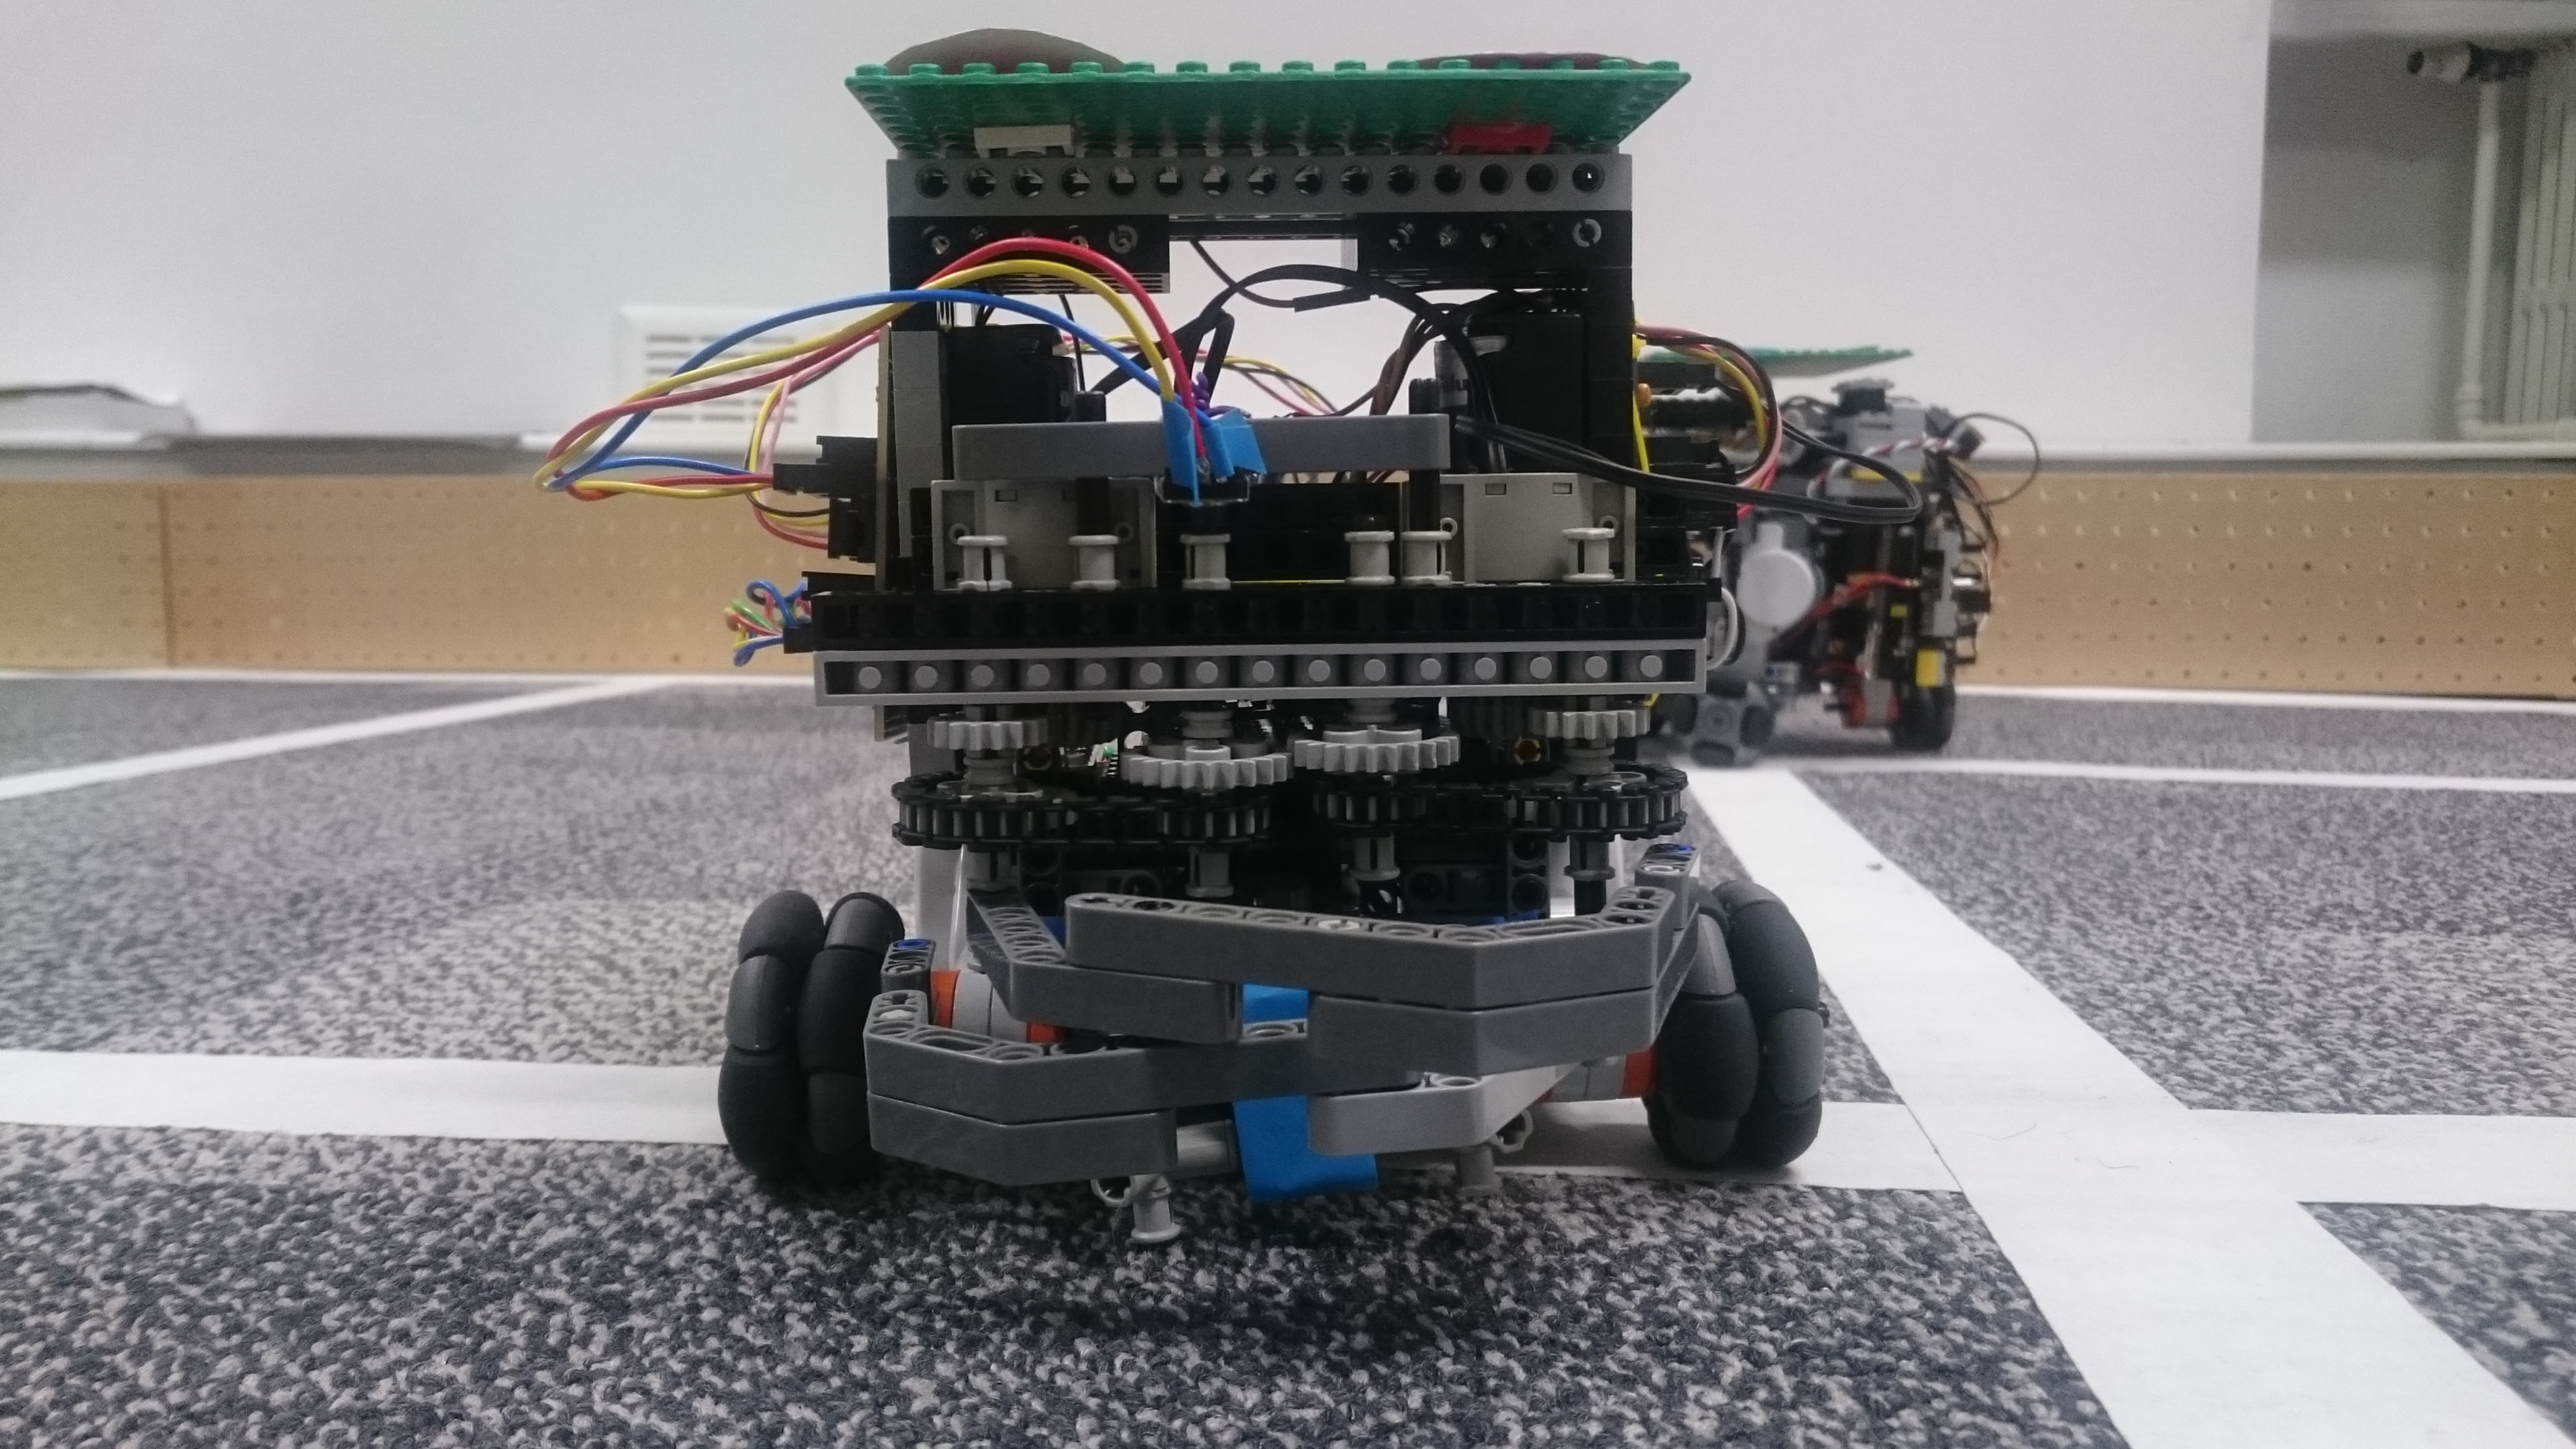
\includegraphics[width=.95\textwidth]{DSC_0031.jpg}
\caption{Front Assembly}
\label{pic:front}
\end{subfigure}
\caption{Robot Construction}
\label{pic:construction}
\end{figure}

\subsection{Wheelbase}
\subsubsection{Dimensions}
'Drive' wheelbase:		15cm \newline
Radius of 'turn' wheel: 11cm
\subsubsection{Origin}
The origin is directly between the 'Drive' wheels
\subsubsection{Arrangement}
The robot uses a 3 wheeled 'T' design with 2 parallel 'drive' wheels along one axis of rotation (capable of rotating independently) and a third unpowered 'turn' wheel rotating perpendicular to these 2 (\autoref{pic:wheelbase}). The 'origin' of the robot should be 
directly between the 2 drive wheels which are 15cm apart. The 'turn' wheel 
is 11cm back from the origin, the left wheel 7.5cm to the left and the right
7.5cm to the right. 

\subsubsection{Motors}
The 2 drive motors are lego NXT motors and have rotational encoders built in, this is used to turn and move accurately. 



\subsection{Front Assembly}
\subsubsection{Description}
The robot Has a 2 motor assembly mounted on 4 vertical bars coming up from the struts joining the left and right NXT drive motors. These are symmetrically mounted and linked by a chain in order to keep them synchronised. The right grabber is lower than the left one so that they do not hit into each other. On one of the centre axles there is a rotary encoder to give the position of the grabbers to the Arduino, through the rotary encoder board. Position 0 is open, 10 is closed with ball and 13 is closed without ball. See \autoref{pic:front}.

The grabber assembly is fully detachable and can be clipped on and off. 


\subsection{Kicker}
\subsubsection{Position}
The kicker is a solenoid mounted on the underside of the robot (see \autoref{pic:construction}) connected through a relay to the battery packs, with the relay signal going to the power shield and being controlled directly by the Arduino. on the end of the solenoid is a curved kicker designed to keep the ball straight.

\subsubsection{Power}
The kicker is capable of kicking a distance of 3.2m at full power with an approx error of 15 percent

\subsection{Board and Battery Assembly}
\subsubsection{Structure}
The boards are mounted on a platform between the 3 wheels. The Arduino and power
shield are mounted in the centre with 2 battery packs of 2 18650 Li-Ion batteries mounted sideways on either
side. The rotary encoder board is
mounted on the back of the right battery pack and the motor driver board is mounted
on the left battery pack. As the batteries face in the packs must be detached to
replace them. Both packs clip onto the platform with lego connectors.

\subsubsection{Batteries}
The batteries are 4* 18650 Canwelum Li-Ion cells wired in series in 2 battery packs. They can be removed and charged individually in the Li-Ion charger.

\begin{table}[H]
\begin{tabularx}{\textwidth}{XX}
\textbf{Voltage (per cell):}	& 2.65 - 4.2 \\
\textbf{Voltage (total):}		& 10.6 - 16.8 \\
\textbf{Max Current:}			& 7A \\
\textbf{Internal Resistance (per cell)}: & 0.150 Ohms \\
\textbf{Internal Resistance (total)}: & 0.6 Ohms \\
\textbf{Capacity}: & 2250mAh \\
\textbf{Protection}: & overvolt and undervolt \\
\end{tabularx}
\end{table}
   
\subsubsection{Connections}
The batteries are connected in series and must be connected to the power board through the yellow switch, with the splitters on the line powering the solenoid relay (orange wires)
\subsubsection{Switch}
A yellow switch turns the robot on and off


\section{Arduino Software}
\subsection{Main Loop}
The main loop listens on the serial port and executes any command received in a non-blocking manner. 
\subsection{Command Set}
The commands are as follows:
kick(distance)
grab()
release()
turn(angle)
move(distance)
\subsection{Command Response}
In response to a command the robot immediately drops what it is doing and runs that command. 
\subsection{Kicking}
The robot releases the grabbers until they are at position 0 then kicks a time dependent on the distance required. It then closes the grabbers to position 13 (fully closed) for continued movement.
\subsection{Grabbing}
The robot closes the grabbers until they are fully closed or 800ms whichever is sooner, if the grabbers only close to position 10 the grab is considered a success and this is sent to the planner. 
\subsection{Release}
The grabbers are released to position 0.
\subsection{Turn}
The robot accelerates up to a calibrated turning speed, then maintains that speed until it has just enough time to decelerate to the required position. The wheels are kept turning the same distance using the distance from the rotary encoders by powering down a motor if it has gone too far and powering it up if it has not gone far enough. The turn is considered finished when the averaged distance from the left and right wheels match the calculated distance required to rotate the desired angle (by using radius of wheels:2.5cm, radius from origin: 7.5cm). 
\subsection{Move}
The robot accelerates up to the calibrated speed and then maintains that speed until it has just enough time to decelerate to the desired distance. It keeps the wheels going the same distance using the rotary encoders by reducing power to a wheel that has gone too far. The distance is determined by $\texttt{radius of the wheels} \times \pi \times \texttt{rotation}$. 


\section{Parts and Costs}

\begin{table}[H]
\caption{Parts and costs}
\begin{tabular}{ l c c c }
Item & Count & Price Each & Total Price \\ \hline
Duplicate keys & 2 & £2.50 & £5 \\
holonomic wheel & 3 & £6 & £18 \\
NXT motor       & 2 & £5 & £10 \\
43362 Electric Technic Mini-Motor 9v & 2 & £0.50 & £1 \\
PED	121-420-610-540, solenoid, tubular, pull, 6V \footref{fnt:solenoid} & 1 & £10.91 & £10.91 \\
Canwelum 18650 protected cells & 8 & £5 & £40 \\
Nitecore charger & 0.5 \footref{fnt:charger} & £14.99 & £7.50 \\
Battery holders & 2 & £3.88 & £7.76 \\
TOTAL & & & £91.17
\end{tabular}
\end{table}

\footlabel{fnt:solenoid}{part is out of production, equivalent part: \url{http://uk.farnell.com/multicomp/mcsmt-1325s12std/solenoid-tubular-push-12v/dp/2008785?CMP=ADV-CRUK-LF}}
\footlabel{fnt:charger}{split between the 2 groups in Team F}

\end{document}
